Occlusion should be handled and objects that disappears by entering something or by becoming stationary should be kept.

\begin{figure}[htb]
	\centering
	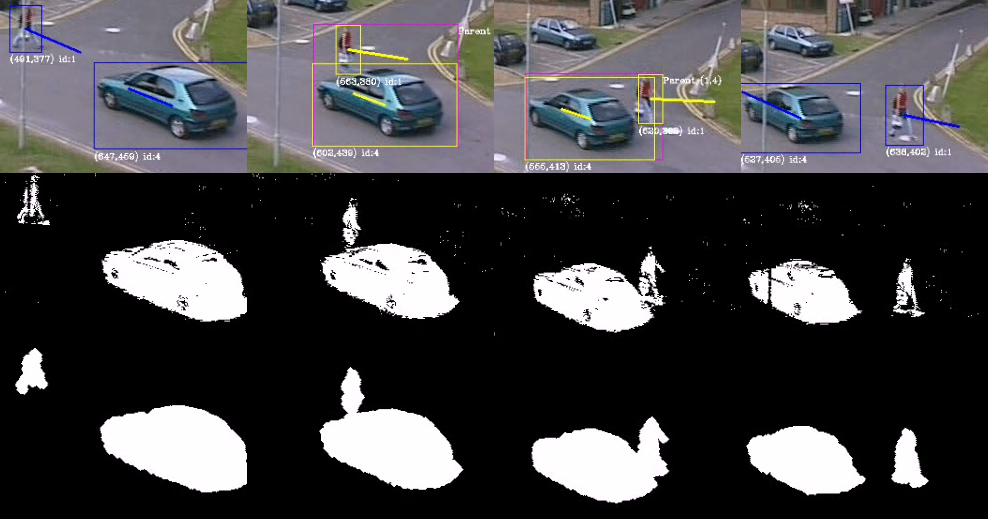
\includegraphics[width=\linewidth]{images/occlusionIllustration1.png}
	\caption{\textit{A part of a sequence from the camera1.mov video illustrating the occlusion handling. Top row is the video with bounding boxes containing different objects, middle row is the thresholded probability map from the background model, bottom row is the result of the foreground segmentation and each connected white blob is a detected object. In the top row: The lines are the estimated velocity multiplied by 30 for visualisation purposes. Single objects are coloured blue, parents are coloured pink, children are coloured yellow.Observe that in the two middle frames only the parent is known and the motion is based on estimates from the Kalman predictions. }}
	\label{fig:UML_fig} %Skapar referens till figuren
\end{figure}

\subsubsection{Situations and solution strategies}
\begin{easylist}
& Two objects (or more) move so close that they are estimated as a single object by the foreground segmentation.
&& The new parent object should not be classified as an object, rather the previous objects should be kept.
&& The old objects should be updated according to their speed vector values of the occlusion moment using the predictor (no measurement update, only time update).
&& The objects should be within the border of the parent object.
&& The objects should only be as wide and high as the parent object, as a maximum restriction.

& An object is moving when it suddenly moves behind a hinder from the background and thus suddenly disappear, then it pop out on the other side of the hinder at a distance from its disappearance.
&& When the object disappear it is marked as lost and is updated according to its speed vector value of the moment of disappearance using the predictor (no measurement update, only time update) until the original object appears close to the estimation. The estimation and the 'new' object is considered the same object.

& An object move in the scene and suddenly stop.
&& The object is marked as lost and kept. When a newly discovered object is close enough it is considered to be the same object.
\end{easylist}
